\begin{center}
    \textbf{\LARGE ĐỀ KIỂM TRA ĐÁNH GIÁ CUỐI BÀI}\\
    \textbf{\Large MÔN: TOÁN 11 -- BỘ SÁCH CÁNH DIỀU / KNTT / CHÂN TRỜI}\\
    \textbf{\large BÀI 22: HAI ĐƯỜNG THẲNG VUÔNG GÓC -- ĐỀ SỐ 01}\\
    \textit{Thời gian làm bài: 45 phút, không kể thời gian phát đề}
\end{center}
\hrule
\vspace{0.5cm}

\noindent\textbf{\large PHẦN I. Câu trắc nghiệm nhiều phương án lựa chọn.} Thí sinh trả lời từ câu 1 đến câu 12. Mỗi câu hỏi thí sinh chỉ chọn một phương án.

\begin{ex}
    Trong không gian, số đo góc giữa hai đường thẳng $a$ và $b$ luôn thuộc đoạn nào dưới đây?
    \choice
    {$(0^\circ; 180^\circ)$}
    {\True $[0^\circ; 90^\circ]$}
    {$[0^\circ; 180^\circ]$}
    {$(0^\circ; 90^\circ)$}
    \loigiai{
        Theo định nghĩa, góc giữa hai đường thẳng trong không gian có số đo từ $0^\circ$ đến $90^\circ$, tức là thuộc đoạn $[0^\circ; 90^\circ]$.
    }
\end{ex}

\begin{ex}
    Cho hai đường thẳng $a$ và $b$ lần lượt có vectơ chỉ phương là $\vec{u}$ và $\vec{v}$. Hai đường thẳng $a$ và $b$ vuông góc với nhau khi và chỉ khi
    \choice
    {\True $\vec{u} \cdot \vec{v} = 0$}
    {$\vec{u} \cdot \vec{v} = 1$}
    {$\vec{u} = k\vec{v}$}
    {$|\vec{u}| = |\vec{v}|$}
    \loigiai{
        Hai đường thẳng vuông góc với nhau khi và chỉ khi tích vô hướng của hai vectơ chỉ phương tương ứng bằng $0$, tức là $\vec{u} \cdot \vec{v} = 0$.
    }
\end{ex}

\begin{ex}
    Trong không gian, khẳng định nào sau đây là \textbf{đúng} về mối quan hệ giữa hai đường thẳng vuông góc?
    \choice
    {Hai đường thẳng vuông góc thì bắt buộc phải cắt nhau}
    {Hai đường thẳng vuông góc thì không thể chéo nhau}
    {Hai đường thẳng vuông góc thì luôn cùng thuộc một mặt phẳng}
    {\True Hai đường thẳng vuông góc có thể cắt nhau hoặc chéo nhau}
    \loigiai{
        Trong không gian, hai đường thẳng vuông góc với nhau có thể cắt nhau (cùng nằm trong một mặt phẳng) hoặc chéo nhau (không cùng thuộc một mặt phẳng).
    }
\end{ex}

\begin{ex}
    Cho ba đường thẳng phân biệt $a, b, c$ trong không gian. Nếu $a \parallel b$ và $c \bot a$ thì
    \choice
    {$c \parallel b$}
    {$c \equiv b$}
    {\True $c \bot b$}
    {$c$ và $b$ trùng nhau}
    \loigiai{
        Theo tính chất: Trong không gian, đường thẳng nào vuông góc với một trong hai đường thẳng song song thì cũng vuông góc với đường thẳng còn lại.
    }
\end{ex}

\begin{ex}
    Một khung vì kèo mái nhà bằng thép tiền chế có dạng tam giác cân $ABC$ ($AB = AC$). Thanh chống đứng $AH$ nối đỉnh $A$ với trung điểm $H$ của xà ngang đáy $BC$. Một thanh xà gồ mái $d$ được lắp đặt song song với xà ngang đáy $BC$.
    \begin{center}
        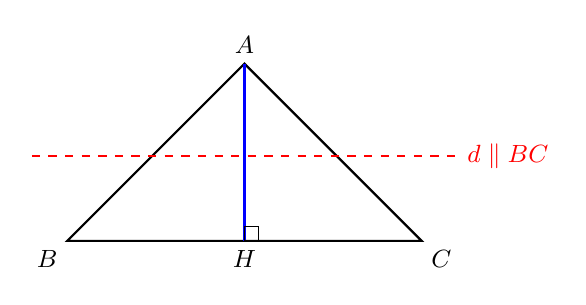
\begin{tikzpicture}[scale=0.9]
            \coordinate (B) at (0,0);
            \coordinate (C) at (5,0);
            \coordinate (H) at (2.5,0);
            \coordinate (A) at (2.5,2.5);
            \draw[thick] (B) -- (A) -- (C) -- cycle;
            \draw[thick, blue] (A) -- (H);
            \draw[thick, dashed, red] (-0.5,1.2) -- (5.5,1.2) node[right] {\small $d \parallel BC$};
            \draw (H) rectangle ++(0.2,0.2);
            \node at (B) [below left] {\small $B$};
            \node at (C) [below right] {\small $C$};
            \node at (A) [above] {\small $A$};
            \node at (H) [below] {\small $H$};
        \end{tikzpicture}
    \end{center}
    Góc giữa thanh chống đứng $AH$ và thanh xà gồ mái $d$ bằng
    \choice
    {\True $90^\circ$}
    {$45^\circ$}
    {$60^\circ$}
    {$30^\circ$}
    \loigiai{
        Vì tam giác $ABC$ cân tại $A$ nên đường trung tuyến $AH$ đồng thời là đường cao, do đó $AH \bot BC$.
        Vì $d \parallel BC$ nên $AH \bot d$, suy ra góc giữa $AH$ và $d$ bằng $90^\circ$.
    }
\end{ex}

\begin{ex}
    Cho hình lập phương $ABCD.A'B'C'D'$. Góc giữa hai đường thẳng $AB$ và $A'C'$ bằng
    \choice
    {$90^\circ$}
    {$60^\circ$}
    {\True $45^\circ$}
    {$30^\circ$}
    \loigiai{
        Do $A'C' \parallel AC$ nên góc giữa $AB$ và $A'C'$ chính là góc giữa $AB$ và $AC$.
        Vì $ABCD$ là hình vuông nên đường chéo $AC$ tạo với cạnh $AB$ một góc $45^\circ$.
        Vậy $(AB, A'C') = 45^\circ$.
    }
\end{ex}

\begin{ex}
    Cho tứ diện đều $ABCD$. Góc giữa hai đường thẳng $AB$ và $CD$ bằng
    \choice
    {$60^\circ$}
    {\True $90^\circ$}
    {$45^\circ$}
    {$30^\circ$}
    \loigiai{
        Trong tứ diện đều, các cặp cạnh đối diện luôn vuông góc với nhau từng đôi một. Do đó $AB \bot CD$, góc giữa chúng bằng $90^\circ$.
    }
\end{ex}

\begin{ex}
    Cho hình chóp $S.ABCD$ có đáy $ABCD$ là hình thoi tâm $O$. Góc giữa hai đường thẳng $AC$ và $BD$ bằng
    \choice
    {$45^\circ$}
    {$60^\circ$}
    {$30^\circ$}
    {\True $90^\circ$}
    \loigiai{
        Đáy $ABCD$ là hình thoi nên hai đường chéo $AC$ và $BD$ vuông góc với nhau tại tâm $O$. Do đó $(AC, BD) = 90^\circ$.
    }
\end{ex}

\begin{ex}
    Một ngọn hải đăng có cột tháp thẳng đứng $SO$ cắm sâu vào nền đá. Một bờ kè bê tông thẳng $d$ chạy dọc chân bờ biển nằm trên mặt phẳng nằm ngang. Góc giữa thân cột hải đăng $SO$ và bờ kè bê tông $d$ bằng
    \choice
    {$45^\circ$}
    {$60^\circ$}
    {\True $90^\circ$}
    {$0^\circ$}
    \loigiai{
        Phương thẳng đứng của cột hải đăng luôn vuông góc với mọi phương nằm ngang trong không gian, do đó góc giữa $SO$ và $d$ bằng $90^\circ$.
    }
\end{ex}

\begin{ex}
    Cho hai đường thẳng $a$ và $b$ có hai vectơ chỉ phương $\vec{u}$ và $\vec{v}$ thỏa mãn $\cos(\vec{u}, \vec{v}) = -\dfrac{1}{2}$. Góc giữa hai đường thẳng $a$ và $b$ bằng
    \choice
    {$120^\circ$}
    {\True $60^\circ$}
    {$30^\circ$}
    {$45^\circ$}
    \loigiai{
        Công thức tính góc giữa hai đường thẳng:
        \[
            \cos(a, b) = |\cos(\vec{u}, \vec{v})| = \left|-\dfrac{1}{2}\right| = \dfrac{1}{2}.
        \]
        Suy ra góc giữa hai đường thẳng là $(a, b) = 60^\circ$.
    }
\end{ex}

\begin{ex}
    Một cầu vượt đường bộ được xây dựng bắc qua tuyến đường sắt bên dưới. Trục đường của cầu vượt và đường ray xe lửa chạy theo hai hướng vuông góc nhau nhưng ở hai cao độ chênh lệch nhau (chéo nhau). Khẳng định nào sau đây là \textbf{đúng}?
    \choice
    {\True Hai đường thẳng chéo nhau và góc giữa chúng bằng $90^\circ$}
    {Hai đường thẳng cắt nhau và góc giữa chúng bằng $90^\circ$}
    {Hai đường thẳng song song với nhau}
    {Hai đường thẳng trùng nhau}
    \loigiai{
        Vì cầu vượt ở phía trên và đường sắt ở phía dưới nên hai trục đường không có điểm chung và không cùng nằm trong một mặt phẳng, tức là chéo nhau. Do hai hướng vuông góc nhau nên góc giữa chúng bằng $90^\circ$.
    }
\end{ex}

\begin{ex}
    Cho hình hộp chữ nhật $ABCD.A'B'C'D'$. Mệnh đề nào sau đây là \textbf{sai}?
    \choice
    {$AB \bot B'C'$}
    {$AA' \bot BC$}
    {$A'D' \bot AB$}
    {\True $AC \bot BD$}
    \loigiai{
        Đáy $ABCD$ của hình hộp chữ nhật là hình chữ nhật nói chung (không nhất thiết là hình vuông), do đó hai đường chéo $AC$ và $BD$ không nhất thiết vuông góc với nhau. Khẳng định $AC \bot BD$ là sai.
    }
\end{ex}

\noindent\textbf{\large PHẦN II. Câu trắc nghiệm đúng sai.} Thí sinh trả lời từ câu 1 đến câu 4. Trong mỗi ý \textbf{a)}, \textbf{b)}, \textbf{c)}, \textbf{d)} ở mỗi câu, thí sinh chọn đúng hoặc sai.

\begin{ex}
    Cho hình lập phương $ABCD.A'B'C'D'$.
    \choiceTFt
    {\True Vectơ chỉ phương của đường thẳng $A'B'$ cùng phương với vectơ $\vec{AB}$}
    {\True Góc giữa hai đường thẳng $A'D'$ và $AB$ bằng $90^\circ$}
    {Góc giữa hai đường thẳng $A'C'$ và $BD$ bằng $60^\circ$}
    {\True Đường thẳng $AA'$ vuông góc với đường thẳng $B'D'$}
    \loigiai{
        \begin{itemchoice}
            \itemch Đúng. Vì $A'B' \parallel AB$ nên hai vectơ chỉ phương tương ứng cùng phương.
            \itemch Đúng. Ta có $A'D' \parallel AD$. Trong hình vuông $ABCD$, $AD \bot AB$ nên $(A'D', AB) = (AD, AB) = 90^\circ$.
            \itemch Sai. Do $A'C' \parallel AC$. Trong hình vuông $ABCD$, hai đường chéo $AC \bot BD$ nên góc giữa $A'C'$ và $BD$ bằng $90^\circ$, không phải $60^\circ$.
            \itemch Đúng. Vì $AA' \parallel BB'$ và $BB' \bot B'D'$ (do $BB' \bot (A'B'C'D')$) nên $AA' \bot B'D'$.
        \end{itemchoice}
    }
\end{ex}

\begin{ex}
    Một cần cẩu tháp trong xây dựng có kết cấu gồm trụ đứng $OT$ thẳng đứng vuông góc với mặt đất, tay cần chính $OA$ vươn dài theo phương nằm ngang và tay cần đối trọng $OB$ nằm thẳng hàng ngược phía với $OA$ ($A, O, B$ thẳng hàng trên mặt phẳng ngang). Dây cáp treo tải hàng $MN$ thả tự do theo phương thẳng đứng.
    \begin{center}
        \begin{tikzpicture}[scale=0.9]
            \draw[thick, gray] (-2,0) -- (5,0);
            \draw[ultra thick, blue!80!black] (0,0) -- (0,4) node[above] {\small $T$};
            \draw[ultra thick, red!80!black] (-1.5,3.2) -- (4,3.2);
            \node at (-1.5,3.2) [left] {\small $B$};
            \node at (0,3.2) [above left] {\small $O$};
            \node at (4,3.2) [right] {\small $A$};
            \draw[thick, dashed] (2.5,3.2) -- (2.5,1.2);
            \node at (2.5,3.2) [above] {\small $M$};
            \node at (2.5,1.2) [below] {\small $N$};
            \fill (0,0) circle (2pt) node[below] {\small Chân cẩu};
            \draw (0,3.2) rectangle ++(0.2,-0.2);
            \draw (2.5,3.2) rectangle ++(-0.2,-0.2);
        \end{tikzpicture}
    \end{center}
    \choiceTFt
    {\True Trục đứng $OT$ vuông góc với cần ngang $AB$}
    {\True Dây cáp treo hàng $MN$ song song với trục đứng $OT$}
    {Góc giữa cần ngang $OA$ và dây cáp treo hàng $MN$ bằng $45^\circ$}
    {\True Khi cần cẩu quay cần ngang $AB$ quanh trục $OT$ thì góc giữa cần ngang $AB$ và dây cáp $MN$ vẫn luôn bằng $90^\circ$}
    \loigiai{
        \begin{itemchoice}
            \itemch Đúng. Trục đứng vuông góc với mặt phẳng nằm ngang chứa cần $AB$ nên $OT \bot AB$.
            \itemch Đúng. Cả trục $OT$ và dây cáp $MN$ đều có phương thẳng đứng nên chúng song song với nhau.
            \itemch Sai. Do $MN \parallel OT$ mà $OT \bot OA$ nên $MN \bot OA$, góc giữa chúng bằng $90^\circ$.
            \itemch Đúng. Khi quay quanh trục đứng, cần ngang $AB$ luôn nằm trong mặt phẳng nằm ngang, trong khi dây cáp $MN$ luôn theo phương thẳng đứng, do đó góc giữa chúng luôn bằng $90^\circ$.
        \end{itemchoice}
    }
\end{ex}

\begin{ex}
    Cho tứ diện $ABCD$ thỏa mãn điều kiện $AB \bot CD$ và $AC \bot BD$.
    \choiceTFt
    {\True Hệ thức vectơ $\vec{CD} = \vec{AD} - \vec{AC}$ là đúng}
    {\True Từ giả thiết $AB \bot CD$, ta suy ra đẳng thức $\vec{AB} \cdot \vec{AD} = \vec{AB} \cdot \vec{AC}$}
    {Cặp cạnh đối diện còn lại $AD$ và $BC$ không vuông góc với nhau}
    {\True Trong một tứ diện, nếu có hai cặp cạnh đối diện vuông góc với nhau thì cặp cạnh đối diện thứ ba cũng vuông góc với nhau}
    \loigiai{
        \begin{itemchoice}
            \itemch Đúng. Theo quy tắc hiệu hai vectơ chung gốc: $\vec{CD} = \vec{AD} - \vec{AC}$.
            \itemch Đúng. Do $AB \bot CD \iff \vec{AB} \cdot \vec{CD} = 0 \iff \vec{AB} \cdot (\vec{AD} - \vec{AC}) = 0 \iff \vec{AB} \cdot \vec{AD} = \vec{AB} \cdot \vec{AC}$.
            \itemch Sai. Tương tự từ $AC \bot BD \implies \vec{AC} \cdot \vec{AD} = \vec{AC} \cdot \vec{AB}$.
            Do đó $\vec{AB} \cdot \vec{AD} = \vec{AC} \cdot \vec{AD} \iff \vec{AD} \cdot (\vec{AB} - \vec{AC}) = 0 \iff \vec{AD} \cdot \vec{CB} = 0 \iff AD \bot BC$.
            \itemch Đúng. Đây là tính chất hình học cơ bản của tứ diện trực tâm: có 2 cặp cạnh đối vuông góc thì cặp cạnh đối thứ ba cũng vuông góc.
        \end{itemchoice}
    }
\end{ex}

\begin{ex}
    Khung chân đế chịu lực của một giàn khoan biển có dạng tứ diện $ABCD$. Các thanh giằng thép có kích thước: $AC = AD = 10\text{ m}$, $BC = BD = 8\text{ m}$, cạnh đáy $CD = 6\text{ m}$ và cạnh trên $AB = 6\text{ m}$. Gọi $M$ là trung điểm của thanh giằng $CD$.
    \choiceTFt
    {\True Tam giác $ACD$ cân tại $A$ nên thanh trung tuyến $AM \bot CD$}
    {\True Tam giác $BCD$ cân tại $B$ nên thanh trung tuyến $BM \bot CD$}
    {Góc giữa hai thanh giằng $AB$ và $CD$ bằng $60^\circ$}
    {\True Độ dài thanh trung tuyến $AM = \sqrt{91}\text{ m}$}
    \loigiai{
        \begin{itemchoice}
            \itemch Đúng. Vì $AC = AD = 10\text{ m}$ nên tam giác $ACD$ cân tại $A$, trung tuyến $AM$ đồng thời là đường cao: $AM \bot CD$.
            \itemch Đúng. Vì $BC = BD = 8\text{ m}$ nên tam giác $BCD$ cân tại $B$, trung tuyến $BM$ đồng thời là đường cao: $BM \bot CD$.
            \itemch Sai. Do $CD \bot AM$ và $CD \bot BM$ nên $CD \bot (ABM)$. Do đó $CD \bot AB$, góc giữa hai thanh $AB$ và $CD$ bằng $90^\circ$.
            \itemch Đúng. Trong tam giác vuông $AMC$ vuông tại $M$: $AM = \sqrt{AC^2 - MC^2} = \sqrt{10^2 - 3^2} = \sqrt{91}\text{ m}$.
        \end{itemchoice}
    }
\end{ex}

\noindent\textbf{\large PHẦN III. Câu trắc nghiệm trả lời ngắn.} Thí sinh trả lời từ câu 1 đến câu 4.

\begin{ex}
    Cho hình lập phương $ABCD.A'B'C'D'$. Tính số đo góc giữa hai đường thẳng $A'B'$ và $B'C$ (đơn vị: độ).
    \shortans{90}
    \loigiai{
        Vì $A'B' \bot B'C'$ và $A'B' \bot B'B$ nên $A'B' \bot (BCC'B')$.
        Mà $B'C$ nằm trong mặt phẳng $(BCC'B')$ nên $A'B' \bot B'C$.
        Vậy góc giữa $A'B'$ và $B'C$ bằng $90^\circ$.
    }
\end{ex}

\begin{ex}
    Cho hình lập phương $ABCD.A'B'C'D'$. Tính số đo góc giữa hai đường thẳng $AC$ và $DA'$ (đơn vị: độ).
    \shortans{60}
    \loigiai{
        Ta có $AC \parallel A'C'$ nên góc giữa $AC$ và $DA'$ bằng góc giữa $A'C'$ và $DA'$.
        Xét tam giác $A'C'D$: các cạnh $A'C', C'D, DA'$ đều là đường chéo của các mặt hình vuông bằng nhau trong hình lập phương.
        Do đó tam giác $A'C'D$ là tam giác đều, suy ra $\widehat{DA'C'} = 60^\circ$.
        Vậy $(AC, DA') = 60^\circ$.
    }
\end{ex}

\begin{ex}
    Một cột đèn chiếu sáng công cộng dựng thẳng đứng trên mặt sân cỏ phẳng. Một vạch sơn thẳng màu trắng được kẻ trên mặt sân cỏ. Biết cột đèn vuông góc với mọi đường thẳng nằm trên mặt sân cỏ. Tính số đo góc giữa cột đèn chiếu sáng và vạch sơn trắng đó (đơn vị: độ).
    \shortans{90}
    \loigiai{
        Vì cột đèn có phương thẳng đứng vuông góc với mặt sân phẳng nên nó vuông góc với vạch sơn trắng nằm trên sân.
        Do đó số đo góc giữa chúng bằng $90^\circ$.
    }
\end{ex}

\begin{ex}
    Cho hình lập phương $ABCD.A'B'C'D'$. Tính số đo góc giữa hai đường thẳng $AB'$ và $BC'$ (đơn vị: độ).
    \shortans{60}
    \loigiai{
        Vì $AB' \parallel DC'$ nên góc giữa $AB'$ và $BC'$ chính là góc giữa $DC'$ và $BC'$.
        Xét tam giác $BDC'$: có ba cạnh $BD, DC', C'B$ là ba đường chéo của ba mặt hình lập phương nên $BD = DC' = C'B$.
        Do đó tam giác $BDC'$ là tam giác đều, suy ra góc $\widehat{BC'D} = 60^\circ$.
        Vậy $(AB', BC') = 60^\circ$.
    }
\end{ex}

\noindent\textbf{\large PHẦN IV. Tự luận.} Thí sinh trả lời từ câu 1 đến câu 2.
\begin{ex}
    Trong một kết cấu giàn vì kèo mái nhà bằng thép, hai thanh thép chịu lực $SA$ và $BC$ chéo nhau trong không gian và vuông góc với nhau. Tính giá trị côsin của góc giữa hai thanh thép đó.
    \loigiai{
        Vì hai thanh thép vuông góc với nhau nên góc giữa chúng bằng $90^\circ$.
        Do đó giá trị côsin của góc giữa hai thanh thép là $\cos 90^\circ = 0$.
    }
\end{ex}

\begin{ex}
    Cho tứ diện $ABCD$ có $AB = CD = 2a$. Gọi $M, N$ lần lượt là trung điểm của hai cạnh $BC$ và $AD$. Biết độ dài đoạn thẳng $MN = a\sqrt{3}$. Tính số đo góc giữa hai đường thẳng $AB$ và $CD$ (đơn vị: độ).
    \loigiai{
        Gọi $P$ là trung điểm của cạnh $AC$.
        Trong tam giác $ABC$, $MP$ là đường trung bình nên $MP \parallel AB$ và $MP = \dfrac{1}{2}AB = a$.
        Trong tam giác $ADC$, $PN$ là đường trung bình nên $PN \parallel CD$ và $PN = \dfrac{1}{2}CD = a$.
        Góc giữa hai đường thẳng $AB$ và $CD$ bằng hoặc bù với góc $\widehat{MPN}$.
        Áp dụng định lý côsin trong tam giác $MNP$:
        \[
            \cos \widehat{MPN} = \dfrac{MP^2 + PN^2 - MN^2}{2 \cdot MP \cdot PN} = \dfrac{a^2 + a^2 - (a\sqrt{3})^2}{2 \cdot a \cdot a} = \dfrac{2a^2 - 3a^2}{2a^2} = -\dfrac{1}{2}.
        \]
        Suy ra $\widehat{MPN} = 120^\circ$.
        Vì góc giữa hai đường thẳng không vượt quá $90^\circ$ nên:
        \[
            (AB, CD) = 180^\circ - 120^\circ = 60^\circ.
        \]
    }
\end{ex}
